\documentclass[12pt]{article}
\usepackage[utf8]{inputenc}
\usepackage{amsmath}
\usepackage{graphicx}
\usepackage[top=1in, bottom=1in, left=1in, right=1in]{geometry}

\title{Trefor Bazett \LaTeX}
\author{Jordan Goff}
\date{}

\begin{document}

\maketitle
\setlength{\parskip}{10pt}
\setlength{\parindent}{0pt}
\newpage

\begin{center}
\section*{Intro to \LaTeX: Learn to write beautiful math equations Part 1}
\end{center}

Hello world! The stuff before the begin document is the preamble. Let's begin with a formula $e^{i\pi}+1=0$. Backslash is a command. A formula with single dollar signs is called an inline formula.

\begin{enumerate} % or itemize for dots.
\item But we can also do
$$e=\lim_{n\to\infty}\left(1+\frac{1}{n}\right)^n=\lim_{n\to\infty}\frac{n}{\sqrt[n]{n!}}.$$

\item We can do another:
$$e=\sum_{n=0}^{\infty}\frac{1}{n!}.$$

\item We can also use continued fractions
$$e=2+\frac{1}{1+\frac{1}{2+\frac{2}{3+\frac{3}{4+\frac{4}{5+\ddots}}}}}.$$
\end{enumerate}

* in front of section will get rid of the number. amsmath gives you multiple integrals, vectors, and matrices. Use \% for comments.

\textbf{More Formulas}
$$\int_{a}^{b}f(x)\,dx$$
$$\iiint f(x,y,z)\,dx\,dy\,dz$$
$$\vec{v}=\langle v_1,v_2,v_3\rangle$$
$$\vec{v}\cdot\vec{w}$$
$$
\begin{bmatrix}
1 & 2 & 3\\
4 & 5 & 6
\end{bmatrix}
$$

\begin{center}
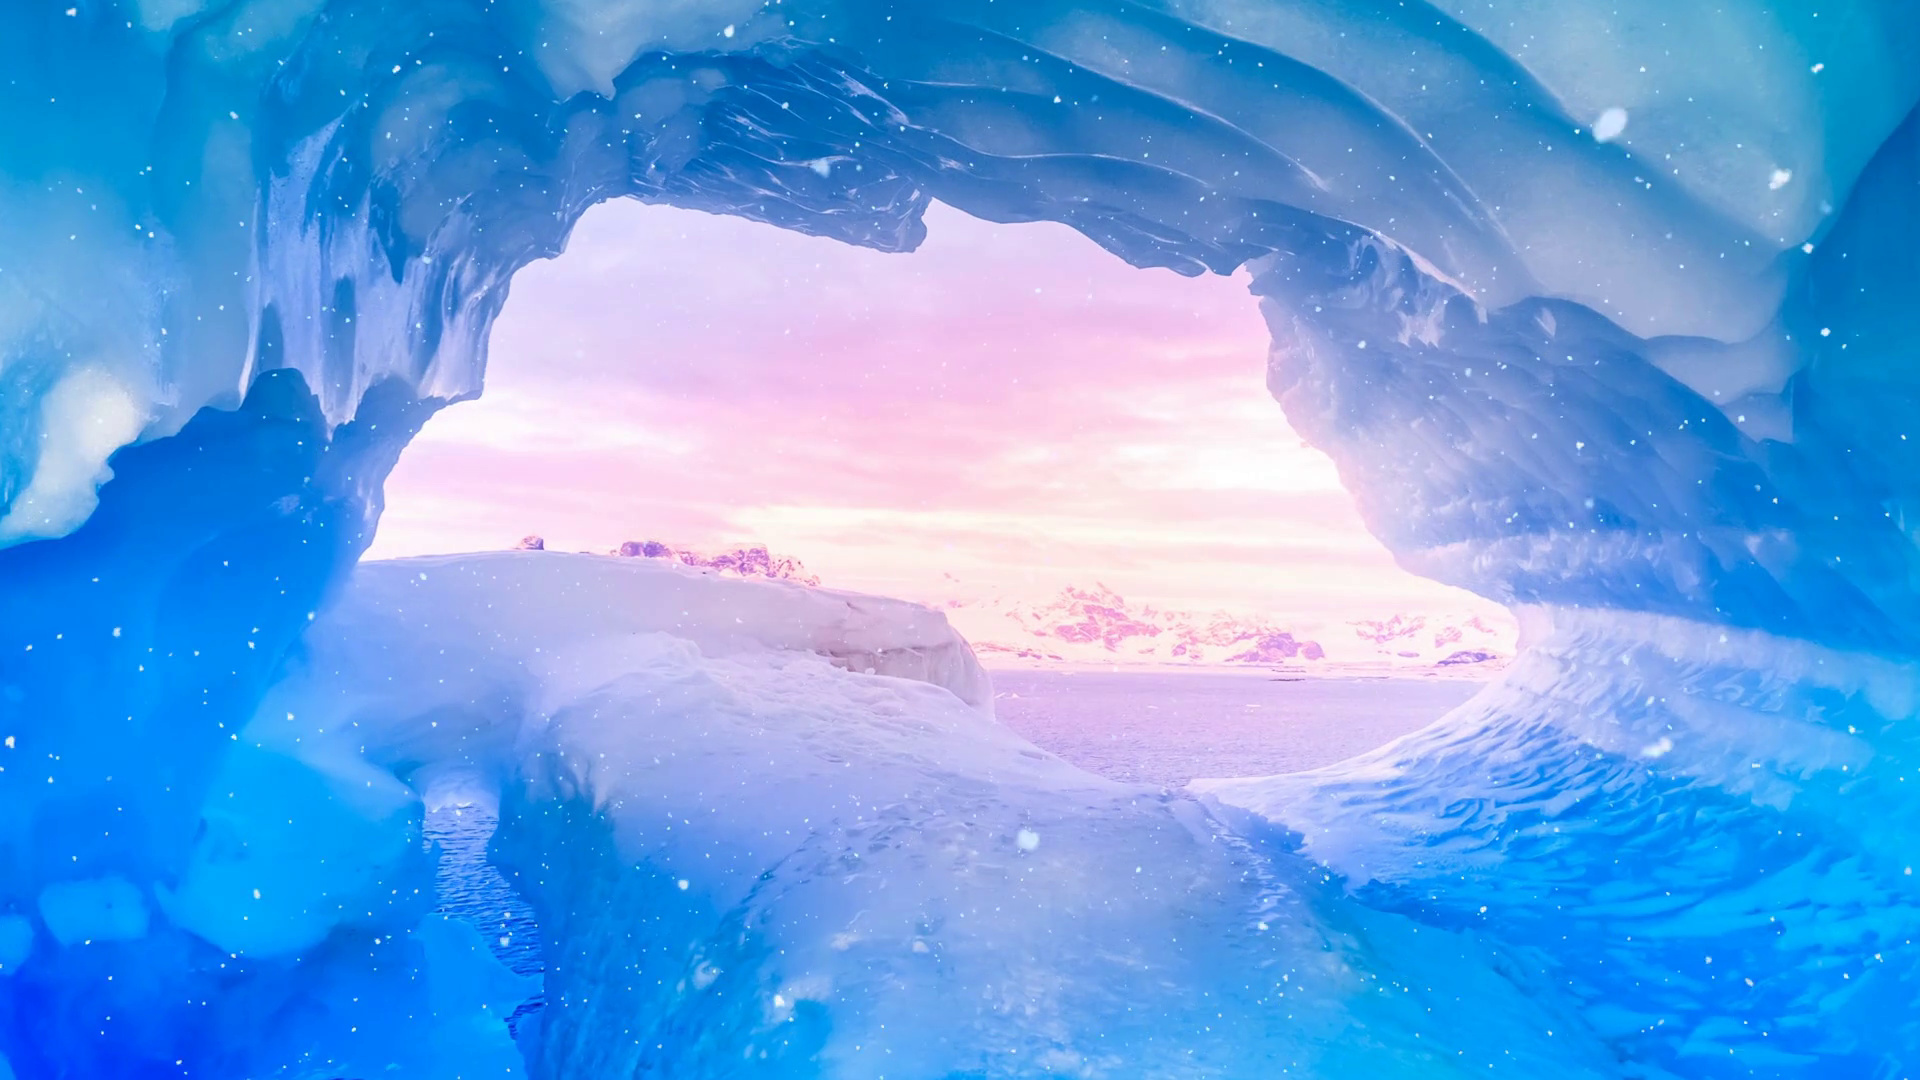
\includegraphics[scale=0.1]{Ice.jpg}
\end{center}

\end{document}